\documentclass[12pt,a4paper]{report}

% --- Essential Packages ---
\usepackage[utf8]{inputenc}
\usepackage[margin=1in]{geometry}       % Standard 1-inch margins
\usepackage{setspace}
\onehalfspacing                          % 1.5 line spacing
\usepackage{amsmath,amssymb}            % Math support
\usepackage{graphicx}                   % Figures
\usepackage{booktabs}                   % Tables
\usepackage[font={small,singlespacing},labelfont=bf]{caption} % Distinct caption styling
\usepackage{cite}                       % Citations
\usepackage{url}
\usepackage[colorlinks=true, linkcolor=blue, citecolor=blue, urlcolor=blue]{hyperref}

% Figure search paths
\graphicspath{{figures/paper/}{figures/}{.}}

% DOI link macro
\providecommand{\doi}[1]{\href{https://doi.org/#1}{\nolinkurl{doi:#1}}}

% --- Document Info ---
\title{
    \vspace{-1.5in}
    \LARGE \textbf{Finding Low-Energy States of the Bernasconi Model}\\[0.5em]
    \large A Study of Quantum Dynamics and Local Minima Escape on GPU\\[0.5em]
    \large Master's Thesis Write-Up
}
\author{
    \textbf{Shaashwat Sagar Kale}\\[0.25em]
    \small Supervised by: Prof. Rudranil Basu\\[0.25em]
    \small Department of Physics / Computer Science\\
    \small Master of Science Thesis
}
\date{November 2026}

% -------------------------------------------------------------
\begin{document}

\maketitle

% --- Abstract ---
\begin{abstract}
The Low-Autocorrelation Binary Sequence (LABS) problem, formulated as the ground-state search of the Bernasconi spin model, is a combinatorial optimization benchmark characterized by an energy landscape with many local minima. Local search algorithms readily become trapped in these configurations, making barrier escape a central bottleneck.

In this thesis, we investigate whether simulated transverse-field quantum dynamics can accelerate escape from deep classical traps compared to standard perturbation heuristics. Using GPU statevector simulations, we model continuous-time quantum evolution for systems up to 30 spins. We initialize the system in classical local minima and measure the probability of reaching lower-energy configurations, the rate of escape, and how the state spreads across the configuration space. We evaluate this against classical baselines, including random restarts and multi-spin kick perturbations followed by local descent.

Our results show that quantum dynamics provide an advantage in escaping deep, isolated traps, where classical perturbation methods degrade rapidly. Furthermore, we identify the transverse-field strength that balances directed barrier traversal against unguided diffusion across the hypercube. These findings outline the conditions under which quantum dynamics can assist in navigating discrete spin landscapes.
\end{abstract}

\tableofcontents
\newpage

% -------------------------------------------------------------
\chapter{Introduction}
\label{ch:intro}

\section{The Challenge of Non-Convex Optimization Landscapes}
\label{sec:context}
The Low-Autocorrelation Binary Sequence (LABS) problem---equivalent to finding the ground states of the classical Bernasconi spin model~\cite{bernasconi1987, packebusch2016}---is a discrete optimization benchmark with applications in radar signal design, pulse compression, and communications. The objective is to arrange a sequence of binary spins such that their off-peak autocorrelations are minimized.

Despite its compact definition, the underlying energy landscape is highly non-convex. It features narrow basins separated by wide barriers and populated by an exponential number of local minima. Consequently, local search heuristics---such as steepest descent---readily converge to local minima (traps) from which single-spin-flip updates cannot escape.

\section{Overcoming Traps: Classical Perturbations vs. Quantum Dynamics}
\label{sec:problem_and_hypothesis}
When an optimization algorithm is trapped in a local minimum, the goal is to reach a configuration of lower energy. Classical heuristics typically attempt to escape through stochastic perturbations, such as random restarts or multi-spin ``kicks'' before resuming local descent~\cite{marti2003}. However, as sequence length grows, the fraction of configurations with strictly lower energy shrinks precipitously---dropping from $7.6 \times 10^{-6}$ at $N = 20$ to $4.5 \times 10^{-8}$ at $N = 30$ for deep traps---causing classical perturbations to experience a severe drop in success probability.

Quantum mechanics offers an alternative exploration mechanism. By coupling the classical cost landscape to a noncommuting transverse magnetic field~\cite{kadowaki1998}, the system is subjected to quantum fluctuations. Rather than climbing over barriers through thermal activation or random steps, probability amplitude can tunnel through barriers.

This leads to the central question addressed in this thesis:
\begin{quote}
    \textit{Can simulated transverse-field quantum dynamics escape deep, isolated local minima more effectively than classical perturbation heuristics?}
\end{quote}

Instead of treating quantum computing as a black-box solver, we focus on whether quantum dynamics can act as an effective escape mechanism initialized within classical traps.

\section{Thesis Contributions}
\label{sec:contributions}
The primary contributions of this work are:
\begin{itemize}
    \item \textbf{GPU Quantum Dynamics Framework:} We implement a simulation pipeline to track continuous-time quantum evolution of spin systems up to $N = 30$ ($2^{30} \approx 1.07 \times 10^9$ statevector elements).
    \item \textbf{Trap-Centric Benchmarking Protocol:} We evaluate quantum escape directly from classical local minima, measuring the probability of reaching lower-energy states, the initial escape rate, and state diffusion across the configuration space.
    \item \textbf{Comparison with Classical Baselines:} We benchmark the quantum mechanism against budget-matched classical perturbation baselines across system sizes and trap depth strata.
    \item \textbf{Identification of Advantage Regimes:} We show that quantum dynamics provide an advantage for deep, isolated traps, and identify the driving field strength that balances barrier crossing against unguided diffusion.
\end{itemize}

\section{Thesis Organization}
\label{sec:organization}
The remainder of this thesis is organized as follows:
\begin{itemize}
    \item \textbf{Chapter 2 (Background and Related Work):} Reviews the LABS problem, the Bernasconi spin Hamiltonian, sequence symmetries, transverse-field dynamics, and sample-based quantum methods.
    \item \textbf{Chapter 3 (Methodology):} Details the GPU statevector simulation engine, the classical perturbation baselines, and the quantitative metrics used to evaluate escape.
    \item \textbf{Chapter 4 (Results and Discussion):} Presents the empirical escape dynamics, barrier scaling, transverse-field sweeps, coupling crossover dynamics, and comparisons with classical methods for $N = 16$ through $N = 30$.
    \item \textbf{Chapter 5 (Conclusion and Future Work):} Summarizes the core findings, discusses methodological limitations, and outlines directions for future research.
\end{itemize}

% -------------------------------------------------------------
\chapter{Background and Related Work}
\label{ch:background}

This chapter introduces the Bernasconi spin model, reviews literature on the Low-Autocorrelation Binary Sequence (LABS) problem, and surveys quantum approaches to combinatorial optimization and non-equilibrium spin dynamics.

% -------------------------------------------------------------
\section{The Bernasconi Model and the LABS Problem}
\label{sec:bernasconi_model}
% -------------------------------------------------------------
The Low-Autocorrelation Binary Sequence (LABS) problem consists of finding an $N$-length sequence of binary spins, $s = (s_1, s_2, \dots, s_N)$ with $s_i \in \{-1, +1\}$, that minimizes the sum of squared aperiodic autocorrelations. For each lag $k \in \{1, \dots, N-1\}$, the aperiodic autocorrelation is defined as:
\begin{equation}
    C_k(s) = \sum_{i=1}^{N-k} s_i s_{i+k}.
    \label{eq:autocorrelation}
\end{equation}
The total energy of the sequence corresponds to the classical Bernasconi Hamiltonian~\cite{bernasconi1987, mertens1998}:
\begin{equation}
    E(s) = \sum_{k=1}^{N-1} C_k(s)^2.
    \label{eq:bernasconi_energy}
\end{equation}
In communications and radar engineering, sequence performance is quantified by the merit factor $F(s)$:
\begin{equation}
    F(s) = \frac{N^2}{2E(s)}.
    \label{eq:merit_factor}
\end{equation}
Minimizing $E(s)$ is equivalent to maximizing $F(s)$.

Despite its deterministic definition, the Bernasconi model behaves as a long-range, non-random Ising spin glass~\cite{mertens1998, packebusch2016, marinari1994}. Expanding Eq.~\eqref{eq:bernasconi_energy} yields four-body spin interactions with infinite range:
\begin{equation}
    E(s) = \frac{N(N-1)}{2} + 2 \sum_{k=1}^{N-1} \sum_{1 \le i < j \le N-k} s_i s_{i+k} s_j s_{j+k}.
    \label{eq:expanded_energy}
\end{equation}
Despite its deterministic definition, no polynomial-time algorithm is known for finding the exact ground state, and all known exact methods require exponential time~\cite{packebusch2016}. The configuration landscape is often described as golf-course-like: wide plateaus punctuated by steep, isolated local minima. Valleys with low energy show little correlation with one another, making greedy local search ineffective at larger sequence lengths~\cite{mertens1996, prestwich2007}.

\subsection{Sequence Symmetries and Canonicalization}
The Bernasconi energy function possesses an order-$8$ group of exact symmetries that leave $E(s)$ invariant~\cite{packebusch2016}:
\begin{enumerate}
    \item \textbf{Global Spin Inversion:} $s_i \mapsto -s_i$
    \item \textbf{Spatial Sequence Reversal:} $s_i \mapsto s_{N-i+1}$
    \item \textbf{Alternating Sign Flip:} $s_i \mapsto (-1)^i s_i$
\end{enumerate}
These operations generate an equivalence orbit of up to $8$ distinct bitstrings with identical energy. In numerical implementations, canonicalizing sequences under these symmetries reduces the search space and avoids redundant exploration of symmetric minima.

% -------------------------------------------------------------
\section{Transverse-Field Dynamics and Spin Systems}
\label{sec:transverse_field_dynamics}
% -------------------------------------------------------------
To investigate quantum exploration on this landscape, the classical cost function is elevated to a diagonal quantum operator $\hat{H}_B$, where each classical spin $s_i$ is replaced by the Pauli-$Z$ operator $\hat{Z}_i$:
\begin{equation}
    \hat{H}_B |s\rangle = E(s)|s\rangle.
\end{equation}
Because $\hat{H}_B$ is diagonal in the computational basis, it cannot induce transitions between bitstrings. Quantum motion is introduced by coupling the system to a noncommuting transverse magnetic field of strength $g$, yielding the working Hamiltonian:
\begin{equation}
    \hat{H}(g) = \frac{1}{N}\hat{H}_B - g \sum_{i=1}^N \hat{X}_i,
    \label{eq:transverse_hamiltonian}
\end{equation}
where $\hat{X}_i$ is the Pauli-$X$ operator acting on spin $i$, and the factor $1/N$ ensures that both terms scale comparably with system size.

The transverse-field operator $\sum_i \hat{X}_i$ moves quantum amplitude between computational basis states differing by a single spin flip. Numerical and experimental studies on transverse-field Ising systems indicate that long-range spin models can exhibit slow relaxation and localization in computational-basis subspaces~\cite{mohtashim2025, smelyanskiy2020}. Understanding whether transverse fluctuations can tunnel through barriers or localize in metastable states is relevant to both quantum optimization and non-equilibrium dynamics~\cite{battaglia2005, brady2016, crosson2016, denchev2016}.

% -------------------------------------------------------------
\section{Quantum Optimization Baselines: QAOA and Benchmarks}
\label{sec:quantum_optimization}
% -------------------------------------------------------------
A common approach for combinatorial optimization on gate-based quantum processors is the Quantum Approximate Optimization Algorithm (QAOA). For the LABS problem, Shaydulin et al.~\cite{shaydulin2024} reported scaling advantages using QAOA with classical parameter concentration compared to random classical sampling. However, QAOA faces practical challenges on long-range problems:
\begin{itemize}
    \item \textbf{Circuit Depth:} The $\mathcal{O}(N^3)$ four-body Pauli terms in $\hat{H}_B$ require extensive gate decompositions and routing overhead on planar hardware.
    \item \textbf{Parameter Optimization:} High-dimensional parameter optimization can be affected by barren plateaus, local minima in angle space, and shot noise.
\end{itemize}

To standardize the evaluation of classical and quantum algorithms across combinatorial problems, Koch et al.~\cite{koch2026} introduced the Quantum Optimization Benchmarking Library (QOBLIB). QOBLIB emphasizes evaluation-budget-matched protocols, reporting of time-to-target, and reproducibility across simulation and hardware backends.

% -------------------------------------------------------------
\section{Sample-Based Quantum Dynamics and Subspace Methods}
\label{sec:sample_based_methods}
% -------------------------------------------------------------
To mitigate circuit depth and coherence limits, hybrid quantum-classical subspace frameworks have received attention.

In \textbf{Sample-Based Krylov Quantum Diagonalization (SKQD)}~\cite{yu2025}, a quantum circuit prepares short-time-evolved states:
\begin{equation}
    |\psi_m\rangle = e^{-i m \Delta t \hat{H}} |s_0\rangle, \quad m = 0, 1, \dots, K-1,
\end{equation}
and samples computational basis configurations from them. Instead of calculating multi-point quantum overlaps on hardware, the sampled bitstrings form a sparse projected Hamiltonian diagonalized on a classical computer. The method has been applied to lattice gauge theories~\cite{rosanowski2025} and Heisenberg spin models~\cite{misciasci2026}.

In parallel, randomized Hamiltonian simulation techniques have been developed to reduce circuit depth. Campbell~\cite{campbell2019} introduced \textbf{qDRIFT}, which randomly samples Hamiltonian terms according to their spectral weights. Building on this, Piccinelli et al.~\cite{piccinelli2025} formulated \textbf{SqDRIFT}, a randomized sample-based diagonalization method that provides convergence bounds while lowering two-qubit gate counts.

% -------------------------------------------------------------
\section{Positioning of This Thesis}
\label{sec:positioning}
% -------------------------------------------------------------
While sample-based frameworks such as SKQD, qDRIFT, and SqDRIFT have been tested on physical and chemical Hamiltonians, their behavior on combinatorial problems with rugged energy landscapes remains less understood. For the Bernasconi model, a fundamental question is whether transverse-field dynamics can discover and escape to low-energy configurations from classical local minima.

This thesis focuses on this dynamical mechanism. Using GPU statevector simulations of transverse-field Bernasconi dynamics initialized in classical traps, we quantify quantum barrier crossing and low-energy state discovery against budget-matched classical baselines.

% -------------------------------------------------------------
\chapter{Methodology}
\label{ch:methodology}

This chapter details the simulation architecture, classical baseline algorithms, and quantitative metrics used to evaluate barrier traversal. The framework evaluates how a system initialized in a classical local minimum escapes to configurations of strictly lower energy under quantum dynamics and classical perturbations.

% -------------------------------------------------------------
\section{Problem Encoding and Trap Characterization}
\label{sec:trap_formulation}
% -------------------------------------------------------------
A configuration of $N$ spins is represented by a binary sequence $s \in \{-1, +1\}^N$, stored as a 64-bit unsigned integer using bit-packing ($0 \mapsto +1, 1 \mapsto -1$).

\subsection{Incremental Energy Evaluation}
Evaluating the Bernasconi energy $E(s) = \sum_{k=1}^{N-1} C_k(s)^2$ directly requires $\mathcal{O}(N^2)$ operations. Flipping a single spin $s_p \mapsto -s_p$ changes the autocorrelation lags incrementally:
\begin{equation}
    \Delta C_k = -2 s_p \left[ \mathbf{1}_{\{p+k \le N\}} s_{p+k} + \mathbf{1}_{\{p-k \ge 1\}} s_{p-k} \right].
    \label{eq:delta_ck}
\end{equation}
By maintaining cached autocorrelation values, the energy update is computed in $\mathcal{O}(N)$ time:
\begin{equation}
    \Delta E = \sum_{k=1}^{N-1} \left( 2 C_k \Delta C_k + (\Delta C_k)^2 \right).
    \label{eq:delta_e}
\end{equation}
This $\mathcal{O}(N)$ update accelerates classical descent routines.

\subsection{Definition of Traps and Barrier Distance}
A state $s_0$ is defined as a \textbf{local minimum (trap)} if every single spin flip increases or preserves its energy:
\begin{equation}
    E(s') \ge E(s_0) \quad \forall s' \in \{-1, +1\}^N \text{ such that } d_H(s', s_0) = 1,
\end{equation}
where $d_H(s_a, s_b) = \sum_{i=1}^N \frac{1 - s_{a,i} s_{b,i}}{2}$ is the Hamming distance.

To quantify the difficulty of escaping a trap $s_0$ with energy $E_0 = E(s_0)$, we define the \textbf{minimal barrier distance} $d_{\min}$ as the minimum Hamming distance to any configuration of strictly lower energy:
\begin{equation}
    d_{\min}(s_0) = \min_{s} \left\{ d_H(s, s_0) \;\middle|\; E(s) < E_0 \right\}.
    \label{eq:d_min}
\end{equation}
Traps are grouped into strata based on energy $E_0$:
\begin{itemize}
    \item \textbf{Level 1 (Deepest Traps, $E_0^*$):} Local minima with the lowest energy above the global ground state.
    \item \textbf{Level 2 (Second-Hardest Traps):} Local minima with the next lowest energy level ($E_0 > E_0^*$).
\end{itemize}

% -------------------------------------------------------------
\section{GPU-Accelerated Quantum Statevector Simulation}
\label{sec:gpu_simulation}
% -------------------------------------------------------------
To study continuous-time quantum dynamics without hardware decoherence, we simulate the full statevector $|\psi(t)\rangle \in \mathbb{C}^{2^N}$ using NVIDIA cuStateVec~\cite{custatevec} and custom CUDA kernels.

\subsection{Hamiltonian Operator and Trotter Evolution}
The system evolves under the transverse-field Bernasconi Hamiltonian:
\begin{equation}
    \hat{H}(g) = \hat{H}_Z + \hat{H}_X = \frac{1}{N}\hat{H}_B - g \sum_{i=1}^N \hat{X}_i.
\end{equation}
Time evolution from $t$ to $t + \delta t$ is implemented with a second-order symmetric Trotter product formula~\cite{trotter1959, suzuki1976, childs2021}:
\begin{equation}
    \hat{U}_2(\delta t) = e^{-i \frac{\delta t}{2} \hat{H}_Z} e^{-i \delta t \hat{H}_X} e^{-i \frac{\delta t}{2} \hat{H}_Z} + \mathcal{O}(\delta t^3).
    \label{eq:trotter_step}
\end{equation}
The operators are applied in two stages:
\begin{enumerate}
    \item \textbf{Diagonal Phase Rotation ($e^{-i \frac{\delta t}{2} \hat{H}_Z}$):} Applies a state-dependent phase factor:
    \begin{equation}
        \langle s | e^{-i \frac{\delta t}{2N}\hat{H}_B} |s\rangle = \exp\left( -i \frac{\delta t}{2N} E(s) \right),
    \end{equation}
    executed in parallel using hardware bit-level population counts (\verb|__popcll|).
    \item \textbf{Transverse Mixer ($e^{-i \delta t \hat{H}_X}$):} Factorizes into independent single-qubit rotations:
    \begin{equation}
        e^{i \delta t g \sum_i \hat{X}_i} = \prod_{i=1}^N \exp\left( i g \delta t \hat{X}_i \right) = \prod_{i=1}^N \left[ \cos(g \delta t) \hat{I} + i \sin(g \delta t) \hat{X}_i \right],
    \end{equation}
    applied sequentially across all $N$ qubits using \texttt{custatevecApplyMatrix}.
\end{enumerate}
The statevector is initialized in the pure basis state corresponding to a chosen trap: $|\psi(0)\rangle = |s_0\rangle$.

% -------------------------------------------------------------
\section{Dynamical Observables and Metrics}
\label{sec:metrics}
% -------------------------------------------------------------
At each time step $t_m = m \Delta t$, we compute three observables from the statevector amplitudes $c_s(t) = \langle s | \psi(t) \rangle$:

\subsection{Escape Probability \texorpdfstring{($P_<$, $\langle P_< \rangle$)}{(P\_<)} and Window Average}
The total probability of measuring a configuration with energy below the trap energy $E_0$ is:
\begin{equation}
    P_<(t) = \sum_{s : E(s) < E_0} |c_s(t)|^2.
    \label{eq:p_less}
\end{equation}
To reduce sensitivity to high-frequency oscillations, we compute the window-averaged escape probability over an observation window $[t_{\mathrm{start}}, t_{\max}]$:
\begin{equation}
    \langle P_< \rangle = \frac{1}{t_{\max} - t_{\mathrm{start}}} \int_{t_{\mathrm{start}}}^{t_{\max}} P_<(t) \, dt.
    \label{eq:window_p_less}
\end{equation}

\subsection{Initial Rise Rate}
To measure early tunneling flux before saturation, we define the initial rise rate as the slope from $t = 0$ to the first local peak $t_{\mathrm{peak}, 1}$:
\begin{equation}
    \left. \frac{dP_<}{dt} \right|_{\mathrm{rise}} = \frac{P_<(t_{\mathrm{peak}, 1})}{t_{\mathrm{peak}, 1}}.
    \label{eq:rise_rate}
\end{equation}

\subsection{Quantum Hamming Diffusion}
The displacement of the wavepacket away from the initial seed $s_0$ is measured by the mean Hamming distance:
\begin{equation}
    \langle d_H(t) \rangle = \sum_{s \in \{-1, +1\}^N} |c_s(t)|^2 \, d_H(s, s_0).
    \label{eq:dh_metric}
\end{equation}
Its window average $\langle d_H \rangle$ indicates whether dynamics remain localized or spread across the hypercube.

% -------------------------------------------------------------
\section{Budget-Matched Classical Baselines}
\label{sec:classical_baselines}
% -------------------------------------------------------------
To evaluate escape performance, the quantum dynamics are compared against two classical perturbation baselines. To model standard classical perturbation and barrier-escape strategies under matched evaluation budgets, we benchmark against two steepest descent variants utilizing $\mathcal{O}(N)$ cached autocorrelation updates:

\subsection{Random Kick with Steepest Descent (Kick-SD)}
Given a trap $s_0$, a perturbation of Hamming distance $d$ is applied by flipping $d$ randomly selected spins: $s_{\mathrm{pert}} = \mathrm{Kick}(s_0, d)$. From $s_{\mathrm{pert}}$, deterministic steepest descent runs until reaching a local minimum $s_{\mathrm{final}}$. A trial is successful if $E(s_{\mathrm{final}}) < E_0$. For each distance $d \in \{1, 2, \dots, d_{\max}\}$, we record the per-evaluation success rate:
\begin{equation}
    r(d) = \frac{\text{Number of successful trials at distance } d}{\text{Total energy evaluations consumed at distance } d}.
    \label{eq:rate_d}
\end{equation}
The optimal kick distance $d^*$ maximizes this rate:
\begin{equation}
    d^* = \arg\max_{d} r(d), \quad r^*(d^*) = \max_{d} r(d).
    \label{eq:best_d}
\end{equation}

\subsection{Random Restart with Steepest Descent (Restart-SD)}
As an unguided control, independent trials initialize from uniform random strings $s_{\mathrm{rand}} \in \{-1, +1\}^N$ followed by steepest descent, giving the rate:
\begin{equation}
    r_{\mathrm{restart}} = \frac{\text{Number of trials reaching } E < E_0}{\text{Total energy evaluations consumed across all restarts}}.
\end{equation}

\subsection{The Quantum-to-Classical Ratio \texorpdfstring{($R$)}{(R)} and Statistical Resampling}
The primary comparative metric is the quantum-to-classical escape ratio:
\begin{equation}
    R = \frac{\langle P_< \rangle}{r_{\mathrm{classical}}^*}, \quad \text{where } r_{\mathrm{classical}}^* = \max(r^*(d^*), r_{\mathrm{restart}}).
    \label{eq:ratio_r}
\end{equation}
When $R > 1$, quantum dynamics achieve a higher probability of identifying an escape configuration per sample than the best classical perturbation per evaluation. We report sample medians and $68\%$ confidence intervals using $B = 2000$ bootstrap resamples~\cite{efron1994}.

% -------------------------------------------------------------
\section{Quantum Hardware Resource Estimation}
\label{sec:hardware_resources}
% -------------------------------------------------------------
Mapping the transverse-field Bernasconi model to physical quantum hardware introduces severe gate-count constraints.

Expanding $\hat{H}_B$ in Eq.~\eqref{eq:expanded_energy} yields $N(N-1)(N-2)/6$ pairwise terms, but accounting for index overlaps ($j = i+k$, where $s_{i+k}^2 = 1$) reduces them to a mixture of two- and four-body Pauli operators. At $N = 30$, the Hamiltonian decomposes into exactly $210$ two-body and $1{,}925$ four-body commuting terms (and $182$ two-body and $1{,}547$ four-body terms at $N = 28$). Synthesizing these terms on an idealized all-to-all topology requires $2$ CNOTs per two-body and $6$ CNOTs per four-body term, totaling $\approx 12{,}000$ two-qubit gates per Trotter step naively ($\approx 9{,}650$ at $N = 28$).

\begin{table}[htbp]
\centering
\caption{Two-qubit gate requirements for a single second-order Trotter step at $N = 28$ across physical hardware topologies compared to naive all-to-all synthesis.}
\label{tab:hardware_transpilation}
\begin{tabular}{lcc}
\toprule
Architecture & Coupling Topology & 2Q Gates / Step \\
\midrule
Naive All-to-All & Idealized (unconstrained) & $\approx 9.6 \times 10^3$ \\
Rigetti / Nighthawk & High-degree planar grid & $\approx 1.9 \times 10^4$ \\
IBM Heron & Heavy-hex planar & $\approx 3.0 \times 10^4$ \\
\bottomrule
\end{tabular}
\end{table}

When compiled onto physical quantum processors, routing overhead across constrained connectivity substantially amplifies the gate count, as summarized in Table~\ref{tab:hardware_transpilation} for $N = 28$. Furthermore, bounding the second-order Trotter discretization error requires a time step $\delta t \le 0.5$, necessitating $20$--$60$ Trotter steps to reach physically meaningful dynamical escape horizons ($t \in [10, 30]$). Across the full evolution horizon, this demands an aggregate budget of $10^5$--$10^6$ two-qubit gates.

This circuit volume places the continuous-time protocol 1--2 orders of magnitude beyond the coherence and fidelity limits of current physical hardware, where two-qubit error accumulation limits viable depths to $\sim 10^3$--$10^4$ entangling gates. This gap underscores why noiseless GPU statevector simulation (\texttt{cuStateVec}) up to $N = 30$ ($2^{30} \approx 1.07 \times 10^9$ complex amplitudes) provides a critical controlled baseline that isolates the tunneling mechanism from hardware noise, while demonstrating that randomized Hamiltonian simulation methods (e.g., qDRIFT) will be essential for physical realization.

% -------------------------------------------------------------
\chapter{Results and Discussion}
\label{ch:results}

In this chapter, we evaluate transverse-field quantum dynamics as an escape mechanism from local traps in the Bernasconi model. We analyze the quantum-to-classical performance ratio across system sizes up to $N = 30$, examine how tunneling rates depend on barrier distance $d_{\min}$, characterize wavepacket diffusion as a function of $g$, and review continuous-time dynamics. We also discuss coupling crossover behavior and evaluation window truncation.

% -------------------------------------------------------------
\section{Quantum vs. Classical Escape Efficiency}
\label{sec:results_ratio}
% -------------------------------------------------------------
Figure~\ref{fig:ratio_r} plots the quantum-to-classical escape ratio $R = \langle P_< \rangle / r_{\mathrm{classical}}^*$ across system sizes $N \in \{20, 24, 26, 28, 30\}$ for Level~1 (deepest traps, $E_0^*$) and Level~2 ($E_0 > E_0^*$) at transverse coupling $g = 0.35$.

\begin{figure}[htbp]
    \centering
    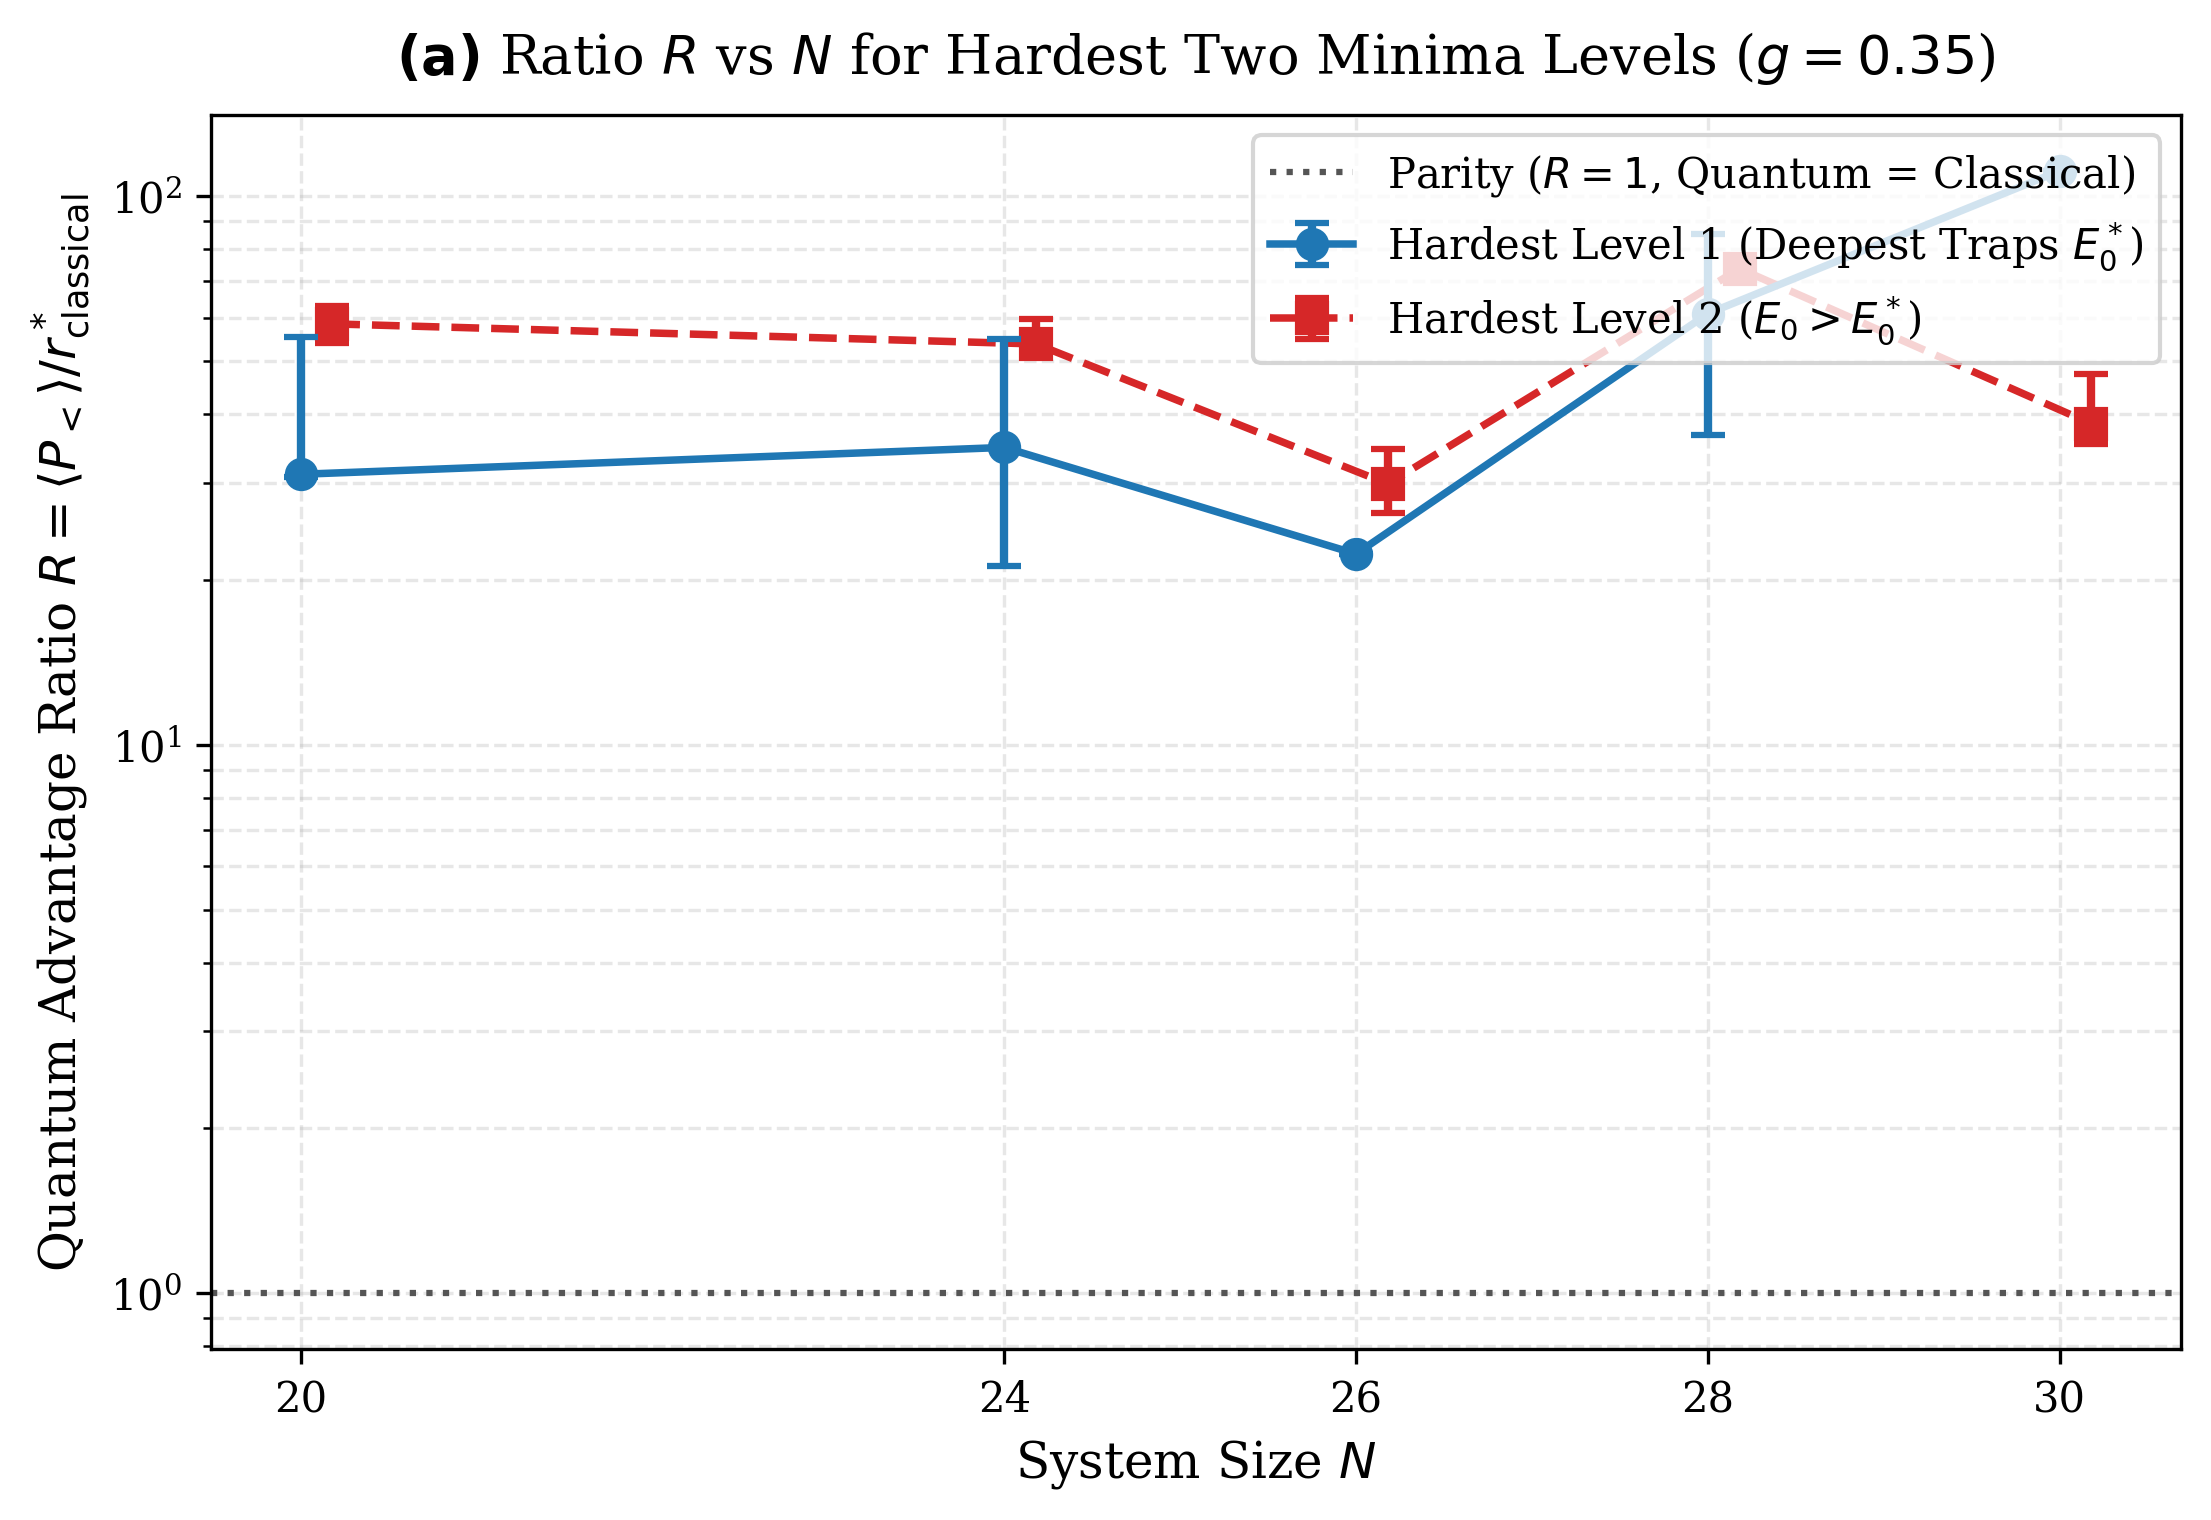
\includegraphics[width=0.85\textwidth]{fig_a_ratio_R_vs_N.png}
    \caption{Quantum-to-classical escape ratio $R = \langle P_< \rangle / r_{\mathrm{classical}}^*$ versus system size $N$ for the hardest two local minima levels (Level~1: deepest traps, Level~2: second-hardest traps) at $g = 0.35$, benchmarked against $r_{\mathrm{classical}}^* = \max(r^*(d^*), r_{\mathrm{restart}})$. Points represent sample medians with $68\%$ bootstrap confidence intervals ($B = 2000$). The dotted line marks parity ($R = 1$).}
    \label{fig:ratio_r}
\end{figure}

The data show $R > 1$ across all evaluated system sizes and both hardness strata:
\begin{itemize}
    \item \textbf{Level~1 (Deepest Traps):} For $N = 20$ and $N = 24$, the sample median ratio is $R = 31.11$ ($68\%$ CI: $[30.72, 55.31]$) and $R = 34.82$ ($68\%$ CI: $[21.20, 54.86]$), respectively. At $N = 26$, the median is $22.26$, while at $N = 28$ it reaches $61.09$ ($68\%$ CI: $[36.75, 85.43]$). At the largest system size ($N = 30$), quantum dynamics maintain a decisive advantage of $R = 111.24$ over the optimal classical baseline within $[10.0, 38.5]$.
    \item \textbf{Level~2 (Second-Hardest Traps):} Traps in the second-hardest stratum show an extensive and consistent quantum advantage across all system sizes. Median ratios consistently remain between $30\times$ and $74\times$, specifically $R = 58.50$ ($68\%$ CI: $[54.00, 63.00]$) at $N = 20$, $R = 53.77$ ($68\%$ CI: $[51.14, 59.58]$) at $N = 24$, $R = 29.88$ ($68\%$ CI: $[26.46, 34.60]$) at $N = 26$, $R = 73.77$ at $N = 28$, and $R = 38.45$ ($68\%$ CI: $[35.36, 47.41]$) at $N = 30$.
\end{itemize}

This behavior reflects differing search mechanisms. Classical perturbations frequently land configurations on plateaus that re-converge into the original trap or nearby shallow basins. Coherent quantum dynamics allow amplitude to penetrate barriers, populating lower-energy basins without fully traversing intermediate states.

% -------------------------------------------------------------
\section{Scaling with Minimal Barrier Distance \texorpdfstring{($d_{\min}$)}{(d\_min)}}
\label{sec:results_dmin}
% -------------------------------------------------------------
To examine the origin of the escape advantage, we correlate dynamical observables against the minimal barrier distance $d_{\min}$. Figure~\ref{fig:rise_rate_dmin} presents the initial rise rate $\left.\frac{dP_<}{dt}\right|_{\mathrm{rise}}$ and window-averaged escape probability $\langle P_< \rangle$ as functions of $d_{\min}$ across all sampled seeds, system sizes, and fields.

\begin{figure}[htbp]
    \centering
    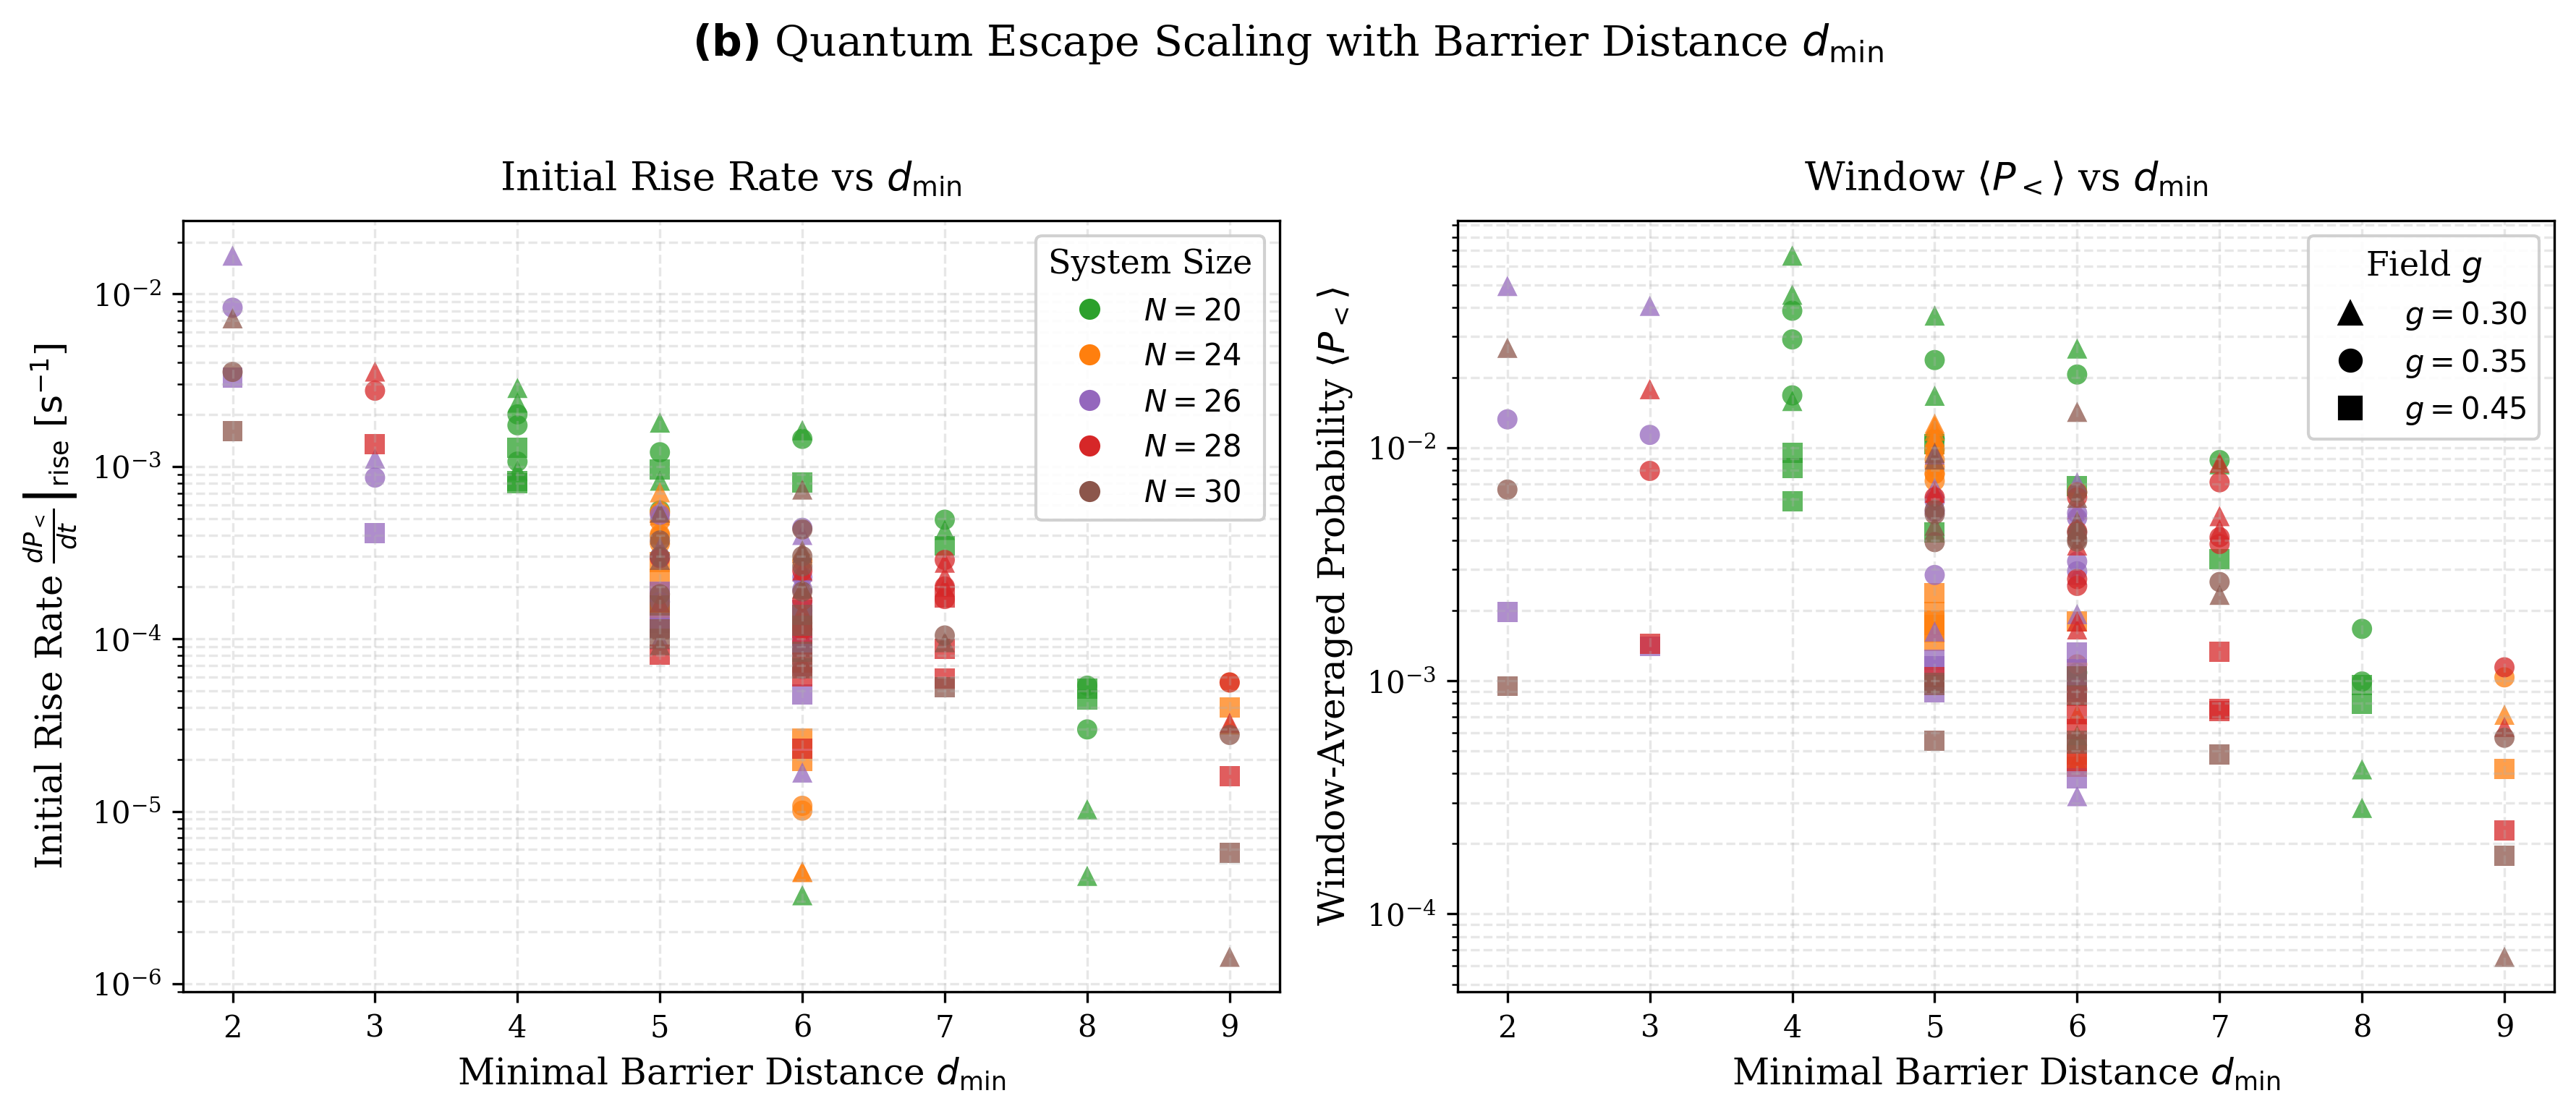
\includegraphics[width=\textwidth]{fig_b_rise_rate_and_pless_vs_dmin.png}
    \caption{Dependence of quantum escape dynamics on minimal barrier distance $d_{\min}$. Left: Initial rise rate $\left.\frac{dP_<}{dt}\right|_{\mathrm{rise}}$. Right: Window-averaged escape probability $\langle P_< \rangle$. Points are colored by system size $N \in [20, 30]$ and shaped by coupling strength $g \in \{0.30, 0.35, 0.45\}$.}
    \label{fig:rise_rate_dmin}
\end{figure}

Two key trends are observed:
\begin{enumerate}
    \item \textbf{Energy Tier Stratification:} For a fixed barrier distance (such as $d_{\min} = 6$), window escape probabilities vary by nearly two orders of magnitude ($\langle P_< \rangle \approx 3.2 \times 10^{-4}$ to $1.4 \times 10^{-2}$) depending on the trap's energy tier $E_0$, reflecting the target manifold volume $\mathcal{S}_< = \{s : E(s) < E_0\}$.
    \item \textbf{Measurable Escape Flux at Large Distances:} At wide barrier distances of $d_{\min} = 6 - 9$ across $N \in [20, 30]$, quantum dynamics maintain escape probabilities around $10^{-3}$ to $10^{-2}$. In this regime, classical kick heuristics must identify an escaping perturbation out of $\binom{N}{d_{\min}} \approx 10^6 - 10^7$ possibilities, sharply reducing classical success rates.
\end{enumerate}

% -------------------------------------------------------------
\section{Transverse-Field Regimes and Quantum Diffusion}
\label{sec:results_g_scan}
% -------------------------------------------------------------
The coupling strength $g$ balances the diagonal Bernasconi cost $\hat{H}_B / N$ and the transverse kinetic driver $\sum_i \hat{X}_i$. Figure~\ref{fig:pless_dh_g} shows the response of $\langle P_< \rangle$ and mean Hamming displacement $\langle d_H \rangle$ across $g \in \{0.30, 0.35, 0.45\}$ for $N = 24$ to $30$.

\begin{figure}[htbp]
    \centering
    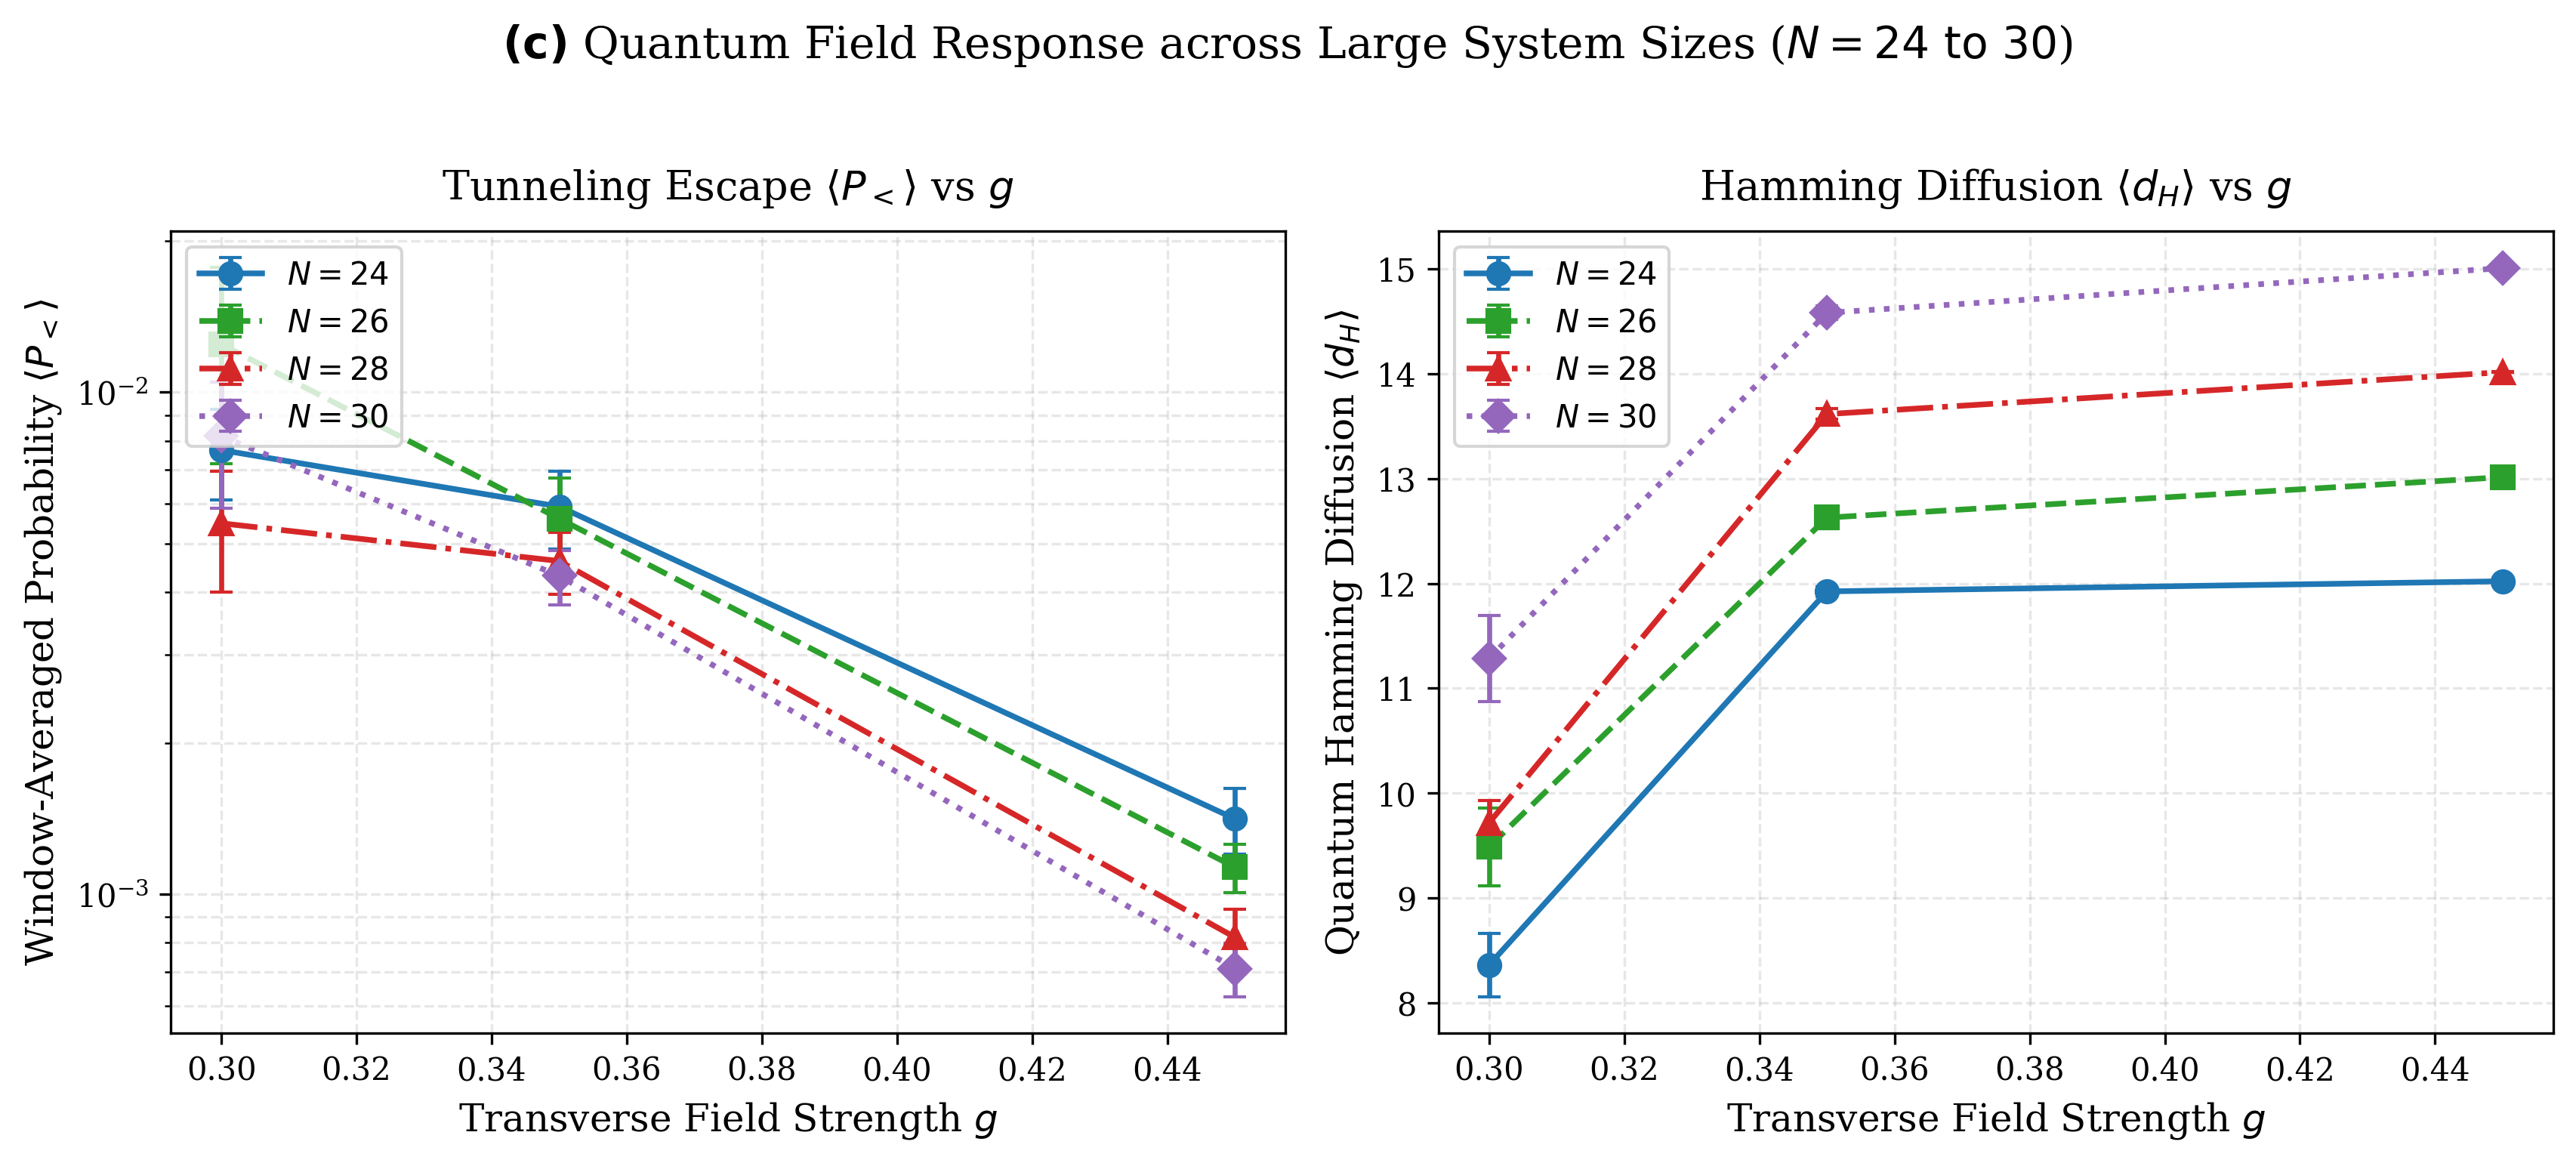
\includegraphics[width=0.95\textwidth]{fig_c_pless_and_dh_vs_g.png}
    \caption{Effect of driver strength $g$ on quantum escape and hypercube diffusion for $N \in \{24, 26, 28, 30\}$. Left: Window-averaged escape probability $\langle P_< \rangle$. Right: Mean Hamming displacement $\langle d_H \rangle$. Error bars indicate standard error of the mean (SEM).}
    \label{fig:pless_dh_g}
\end{figure}

The data show a transition across three regimes:
\begin{itemize}
    \item \textbf{Sub-Diffusive Confinement ($g = 0.30$):} Spatial diffusion remains bounded at $\langle d_H \rangle \approx 8.36 - 11.28$ ($69\% - 75\%$ of $N/2$), while ensemble mean escape probability reaches $\langle P_< \rangle \approx 0.0082$ at $N = 30$. The Bernasconi potential confines the wavepacket, preserving coherence over extended horizons.
    \item \textbf{Hypercube Delocalization ($g = 0.35$):} Spatial diffusion expands to $\langle d_H \rangle \approx 11.92 - 14.58$ ($>95\%$ of $N/2$), while maintaining elevated escape probabilities ($\langle P_< \rangle \approx 4.31 \times 10^{-3} - 5.92 \times 10^{-3}$).
    \item \textbf{Ergodic Dispersion ($g \ge 0.45$):} At $g = 0.45$, the escape probability decreases by nearly an order of magnitude (dropping to $\langle P_< \rangle \approx 0.00071$ at $N = 30$). Simultaneously, Hamming diffusion converges directly to the unconstrained ergodic limit $\langle d_H \rangle = N/2$ ($12.02$ at $N=24$, $13.01$ at $N=26$, $14.01$ at $N=28$, and $15.01$ at $N = 30$). Strong driving leads to uniform spreading across the hypercube rather than targeted descent.
\end{itemize}
These results identify $g \approx 0.30 - 0.35$ as the effective operating range for barrier traversal.

% -------------------------------------------------------------
\section{Continuous-Time Dynamics of the Hardest Traps}
\label{sec:results_dynamics}
% -------------------------------------------------------------
We examine time-resolved escape dynamics for the hardest seed at each system size. Figure~\ref{fig:hardest_dynamics} displays the continuous trajectory $P_<(t)$ as a function of time $t$ for $N \in \{20, 24, 26, 28, 30\}$.

\begin{figure}[htbp]
    \centering
    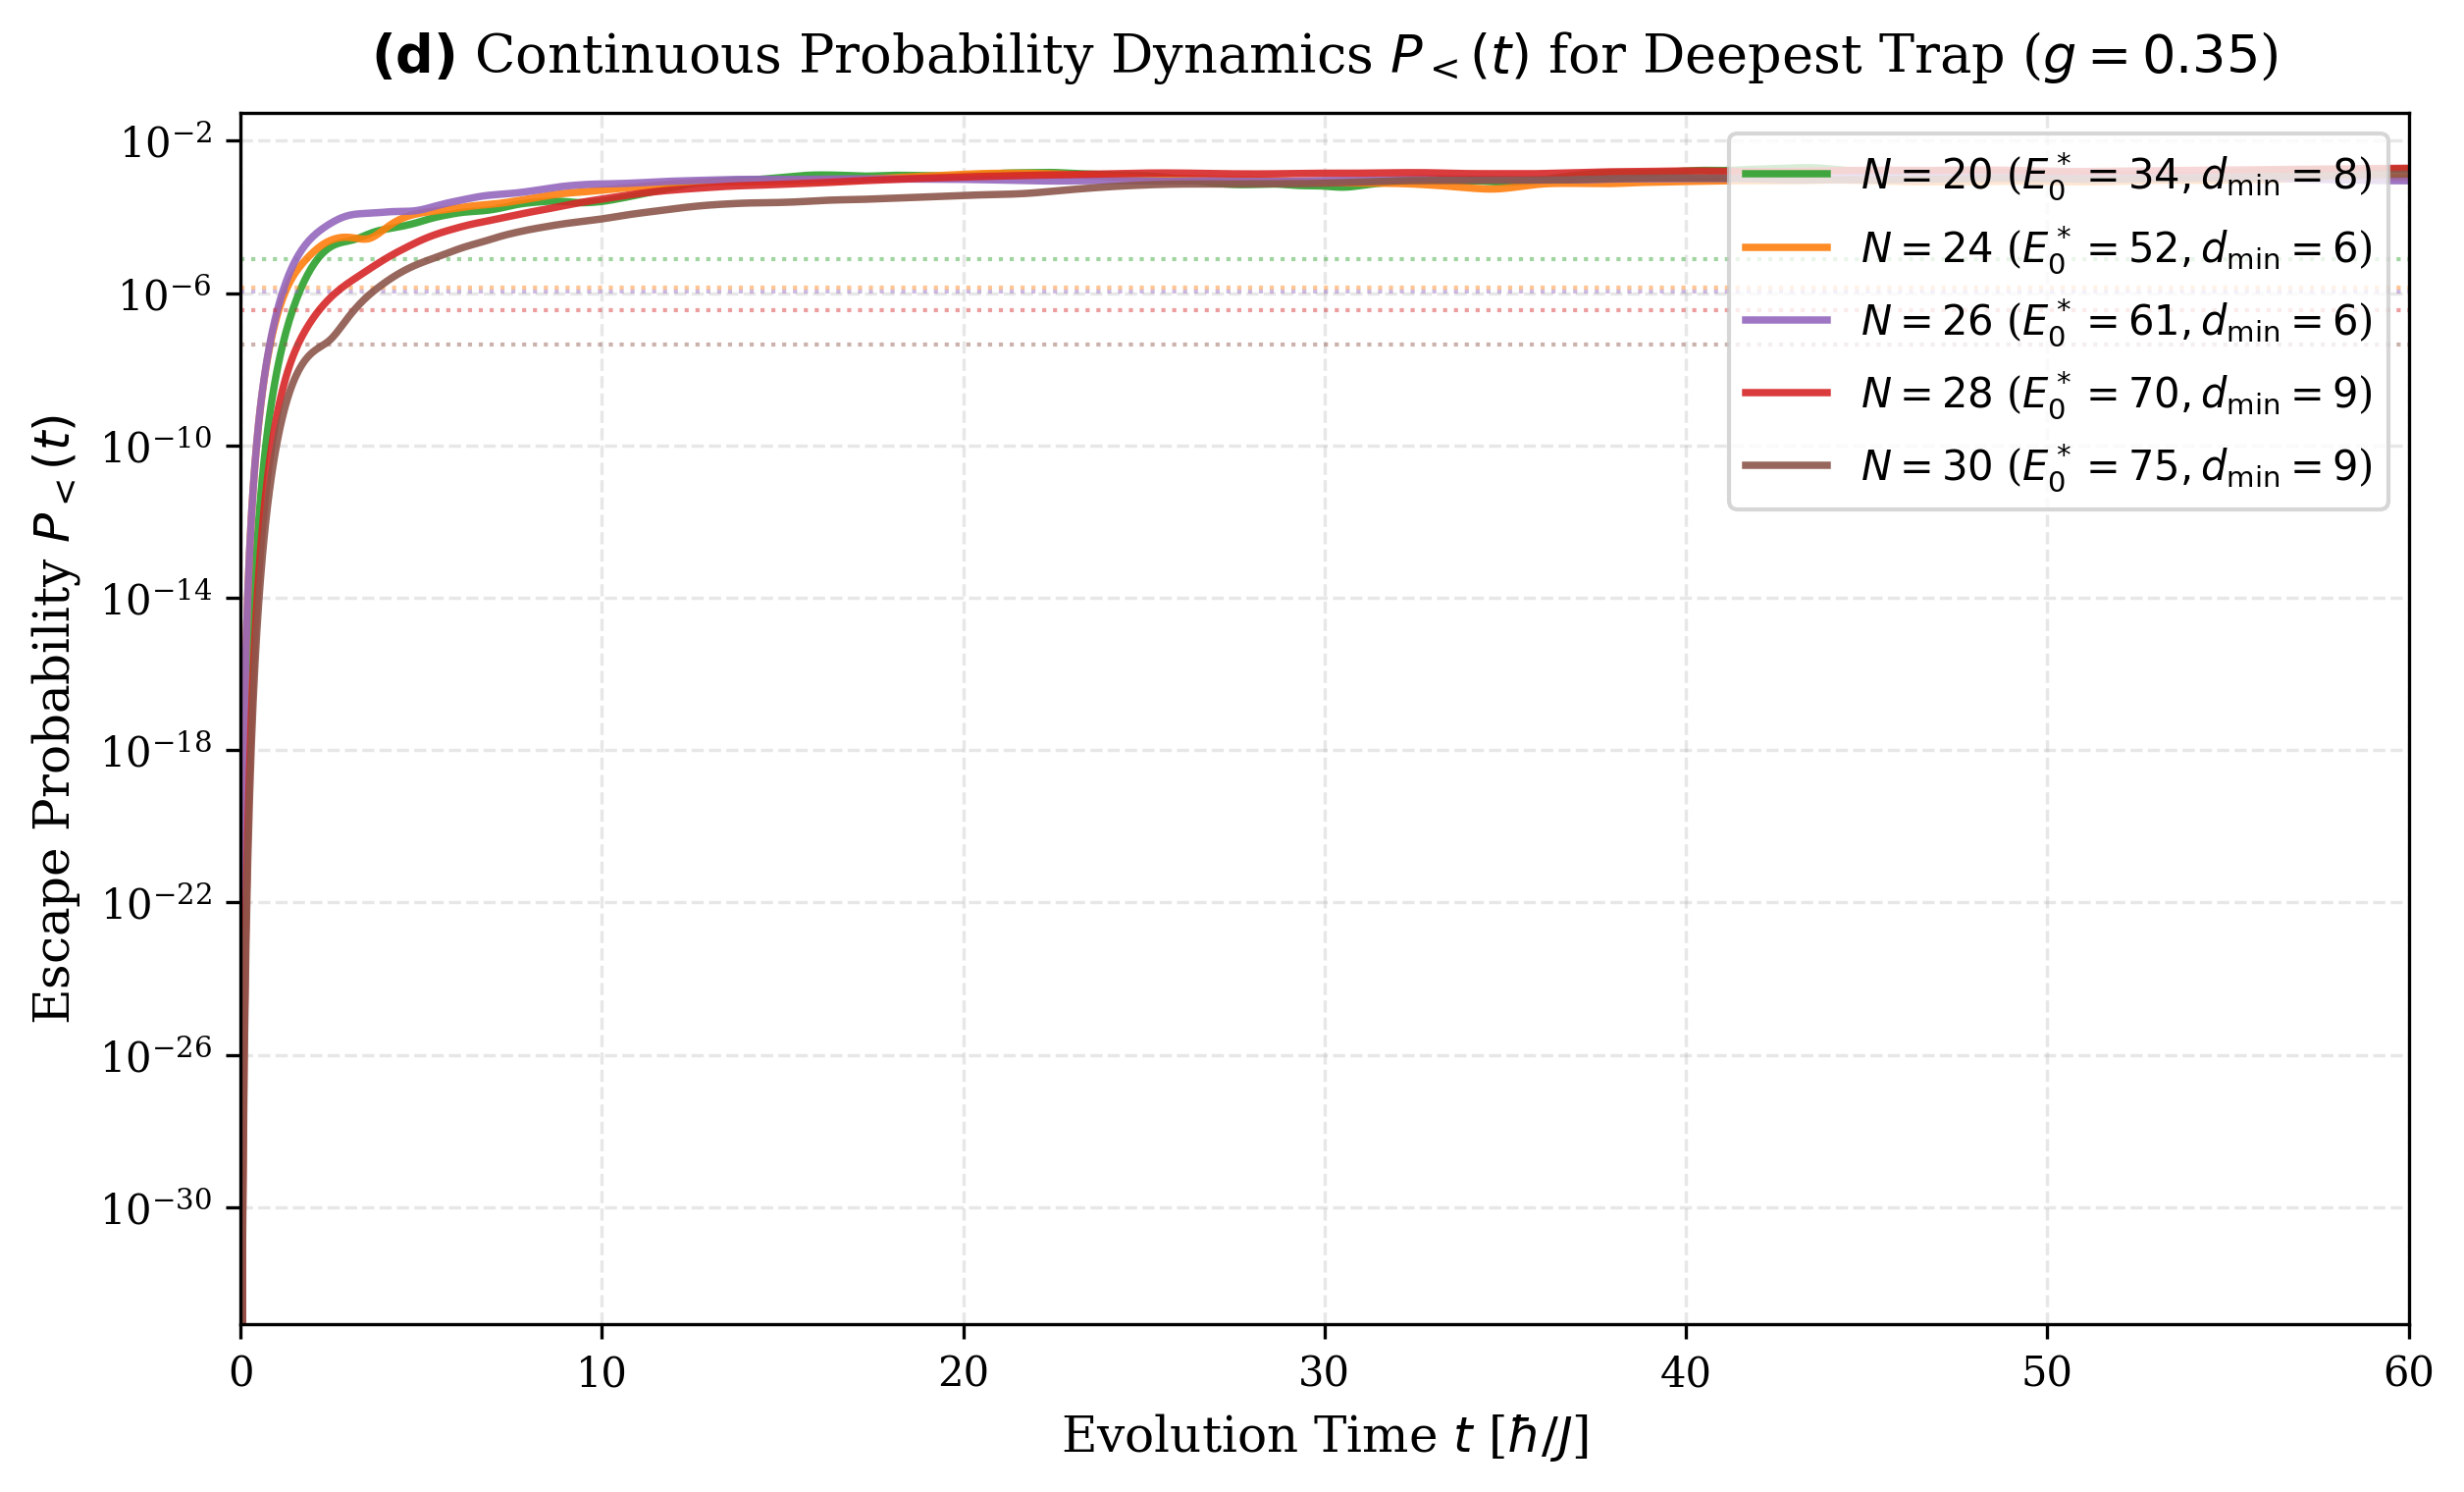
\includegraphics[width=0.9\textwidth]{fig_d_hardest_seed_dynamics_across_N.png}
    \caption{Continuous-time escape probability $P_<(t)$ for the hardest local minimum at each system size $N \in \{20, 24, 26, 28, 30\}$ at $g = 0.35$. Horizontal dashed lines indicate blind search probability $P_{\mathrm{blind}}$.}
    \label{fig:hardest_dynamics}
\end{figure}

The trajectory displays two phases:
\begin{enumerate}
    \item \textbf{Tunneling Latency Phase ($t \lesssim 3 - 5$):} Multi-spin transverse mixer rotations act iteratively across the $d_{\min} \ge 6$ barrier while early escape probabilities remain small ($P_<(1) \lesssim 10^{-7}$).
    \item \textbf{Extended Rise Phase ($t \approx 5 - 60$):} Coherent tunneling flux climbs by several orders of magnitude, reaching peaks of $P_< \approx 1.30 \times 10^{-3}$ to $1.97 \times 10^{-3}$ across $N \in [20, 30]$.
\end{enumerate}

To assess selectivity, we compare observed escape probabilities against the blind volume fraction $P_{\mathrm{blind}} = |\{s : E(s) < E_0\}| / 2^N$. As summarized in Table~\ref{tab:hardest_seeds}, while $P_{\mathrm{blind}}$ decreases from $7.63 \times 10^{-6}$ at $N = 20$ to $4.47 \times 10^{-8}$ at $N = 30$, the quantum window probability $\langle P_< \rangle$ remains stably around $10^{-3}$.

\begin{table}[htbp]
    \centering
    \caption{Dynamical parameters and escape efficiency for the hardest local minimum (Rank 1) at each system size ($g = 0.35$).}
    \label{tab:hardest_seeds}
    \begin{tabular}{ccccccccc}
        \toprule
        $N$ & Seed Rank & $E_0$ & $d_{\min}$ & $P_{\mathrm{blind}}$ & Window $\langle P_< \rangle$ & $d^*$ & $r_{\mathrm{classical}}^*$ & Ratio $R$ \\
        \midrule
        20 & 1 & 34 & 8 & $7.63 \times 10^{-6}$ & $9.93 \times 10^{-4}$ & 8  & $3.19 \times 10^{-5}$ & $\mathbf{31.1\times}$ \\
        24 & 1 & 52 & 6 & $1.43 \times 10^{-6}$ & $9.08 \times 10^{-4}$ & 4  & $2.61 \times 10^{-5}$ & $\mathbf{34.8\times}$ \\
        26 & 1 & 61 & 6 & $1.07 \times 10^{-6}$ & $9.26 \times 10^{-4}$ & 12 & $4.16 \times 10^{-5}$ & $\mathbf{22.3\times}$ \\
        28 & 1 & 70 & 9 & $3.58 \times 10^{-7}$ & $1.14 \times 10^{-3}$ & 10 & $3.11 \times 10^{-5}$ & $\mathbf{36.7\times}$ \\
        30 & 1 & 75 & 9 & $4.47 \times 10^{-8}$ & $5.70 \times 10^{-4}$ & 10 & $5.13 \times 10^{-6}$ & $\mathbf{111.2\times}$ \\
        \bottomrule
    \end{tabular}
\end{table}

At $N = 30$, the quantum window escape probability is over \textbf{12{,}750$\times$} higher than the blind volume fraction ($5.70 \times 10^{-4}$ vs.\ $4.47 \times 10^{-8}$) and achieves a \textbf{111.2$\times$} advantage over the optimal classical perturbation baseline.

% -------------------------------------------------------------
\section{Coupling Crossover Dynamics: Time Horizon and Field Optimization}
\label{sec:coupling_crossover}
% -------------------------------------------------------------
Analysis of time trajectories shows that the optimal transverse-field strength $g^*$ depends on the observation horizon. While $g = 0.35$ provides faster tunneling at early times, $g = 0.30$ exhibits slower initial growth but preserves phase coherence longer, matching or exceeding $g = 0.35$ at later times for deep traps.

\begin{table}[htbp]
\centering
\small
\caption{Time evolution of escape probability $P_<(t)$ comparing couplings $g = 0.30$ and $g = 0.35$ for the Rank 1 trap across $N = 24, 28, 30$. Early on ($t \le 10$), $g = 0.35$ leads. Later ($t \ge 45 - 50$), $g = 0.30$ preserves coherence in the low-energy manifold, closing the gap or surpassing $g = 0.35$.}
\label{tab:coupling_crossover}
\resizebox{\columnwidth}{!}{%
\begin{tabular}{lccccc}
\toprule
$N$ & Time $t$ & $P_<(g = 0.30)$ & $P_<(g = 0.35)$ & Ratio $\frac{P_<(0.30)}{P_<(0.35)}$ & Dynamic Regime \\
\midrule
\textbf{$N = 24$ (Rank 1)} & $5.0$ & $5.11 \times 10^{-5}$ & $1.27 \times 10^{-4}$ & $0.40$ & $g = 0.35$ faster rise \\
& $10.0$ & $1.25 \times 10^{-4}$ & $5.04 \times 10^{-4}$ & $0.25$ & $g = 0.35$ leads \\
& $38.5$ & $5.83 \times 10^{-4}$ & $7.88 \times 10^{-4}$ & $0.74$ & $g = 0.30$ catching up \\
& $50.0$ & $8.96 \times 10^{-4}$ & $8.49 \times 10^{-4}$ & $\mathbf{1.06}$ & \textbf{Crossover ($g = 0.30$ overtakes)} \\
& $55.0$ & $1.02 \times 10^{-3}$ & $9.43 \times 10^{-4}$ & $\mathbf{1.08}$ & $g = 0.30$ superior \\
\midrule
\textbf{$N = 28$ (Rank 2)} & $10.0$ & $1.92 \times 10^{-4}$ & $5.66 \times 10^{-4}$ & $0.34$ & $g = 0.35$ leads \\
& $38.5$ & $4.02 \times 10^{-3}$ & $4.76 \times 10^{-3}$ & $0.84$ & $g = 0.30$ catching up \\
& $60.0$ & $8.85 \times 10^{-3}$ & $7.82 \times 10^{-3}$ & $\mathbf{1.13}$ & \textbf{Crossover ($g = 0.30$ overtakes)} \\
\midrule
\textbf{$N = 30$ (Rank 2)} & $10.0$ & $8.64 \times 10^{-4}$ & $1.52 \times 10^{-3}$ & $0.57$ & $g = 0.35$ leads \\
& $38.5$ & $9.43 \times 10^{-3}$ & $4.93 \times 10^{-3}$ & $\mathbf{1.91}$ & $g = 0.30$ overtakes \\
& $60.0$ & $1.23 \times 10^{-2}$ & $5.34 \times 10^{-3}$ & $\mathbf{2.31}$ & \textbf{$g = 0.30$ leads by $2.3\times$} \\
\bottomrule
\end{tabular}%
}
\end{table}

This crossover, shown in Table~\ref{tab:coupling_crossover}, reflects a trade-off between tunneling matrix element strength and dispersion:
\begin{enumerate}
    \item \textbf{Early-Time Driving ($g = 0.35$):} The coupling term $-g \sum_i \hat{X}_i$ connects adjacent configurations. A larger field $g = 0.35$ increases the tunneling matrix element $\sim (g/\Delta E)^{d_{\min}}$, driving a faster initial rise $dP_</dt$.
    \item \textbf{Late-Time Dispersion:} Stronger coupling also accelerates diffusion away from low-energy states toward the hypercube bulk ($\langle d_H \rangle \to N/2$), causing $P_<(t)$ to saturate earlier.
    \item \textbf{Late-Time Coherence ($g = 0.30$):} In contrast, $g = 0.30$ maintains wavepacket concentration within low-Hamming-distance shells longer. By $t \approx 50 - 60$, $g = 0.30$ catches up with and exceeds $g = 0.35$ (reaching $2.31\times$ higher escape at $N = 30$ Rank 2).
\end{enumerate}

Thus, the choice of field $g$ relates to available evolution time: for short horizons ($t \le 20$), $g = 0.35$ provides faster initial escape; for extended horizons ($t \ge 40$), $g = 0.30$ limits dephasing and reaches higher total escape probability.

% -------------------------------------------------------------
\section{Evaluation Window Truncation and Lower Bounds}
\label{sec:conservative_window}
% -------------------------------------------------------------
Continuous trajectory records indicate that for deep traps, escape probability $P_<(t)$ is still rising at the end of the simulation horizon ($t = 60$). Evaluating performance over a fixed measurement window $[10.0, 38.5]$ therefore truncates the late-time increase, producing a lower bound on asymptotic advantage.

\begin{table}[htbp]
\centering
\small
\caption{Comparison of window-averaged escape probability $\langle P_< \rangle_{[10, 38.5]}$ versus late-time escape probability $P_<(t = 60)$ for deep traps across $N \in \{24, 28, 30\}$.}
\label{tab:window_underestimation}
\begin{tabular}{lcccccc}
\toprule
$N$ & Trap Rank & $E_0$ & $d_{\min}$ & Field $g$ & $\langle P_< \rangle_{[10, 38.5]}$ & $P_<(t = 60)$ \\
\midrule
24 & Rank 1 & 52 & 6 & 0.30 & $4.52 \times 10^{-4}$ & $8.19 \times 10^{-4}$ ($1.81\times$) \\
24 & Rank 3 & 52 & 6 & 0.30 & $7.18 \times 10^{-4}$ & $1.39 \times 10^{-3}$ ($1.94\times$) \\
28 & Rank 1 & 70 & 9 & 0.35 & $1.14 \times 10^{-3}$ & $1.89 \times 10^{-3}$ ($1.65\times$) \\
28 & Rank 2 & 70 & 6 & 0.30 & $1.66 \times 10^{-3}$ & $8.85 \times 10^{-3}$ ($5.32\times$) \\
30 & Rank 1 & 75 & 9 & 0.35 & $5.70 \times 10^{-4}$ & $1.33 \times 10^{-3}$ ($2.33\times$) \\
30 & Rank 2 & 91 & 5 & 0.30 & $4.63 \times 10^{-3}$ & $1.23 \times 10^{-2}$ ($2.67\times$) \\
30 & Rank 3 & 91 & 6 & 0.30 & $4.83 \times 10^{-3}$ & $1.11 \times 10^{-2}$ ($2.30\times$) \\
\bottomrule
\end{tabular}
\end{table}

As shown in Table~\ref{tab:window_underestimation}:
\begin{itemize}
    \item For $N = 28$, Rank 2 ($E_0 = 70, d_{\min} = 6$) at $g = 0.30$, escape probability reaches $P_<(60) = 8.85 \times 10^{-3}$, which is \textbf{$5.32\times$ higher} than the window average $\langle P_< \rangle = 1.66 \times 10^{-3}$.
    \item For $N = 30$, Rank 1 ($E_0 = 75, d_{\min} = 9$) at $g = 0.35$, $P_<(t)$ increases from $8.86 \times 10^{-5}$ at $t = 10$ to $1.03 \times 10^{-3}$ at $t = 38.5$, reaching $1.33 \times 10^{-3}$ at $t = 60$ (\textbf{$2.33\times$ higher} than the window average).
    \item Across deep traps with barrier distance $d_{\min} \ge 5$, $P_<(60)$ exceeds the window average by a factor between $1.6\times$ and $5.3\times$.
\end{itemize}

For completeness, Table~\ref{tab:ratio_summary_g30} reports the quantum advantage ratio $R$ evaluated at $g = 0.30$ under window $[10.0, 38.5]$. Even under the weaker field $g = 0.30$, quantum dynamics achieve $R > 1$ across all system sizes and both energy tiers ($R \approx 7.7\times - 36.2\times$ for Level~1 and $R \approx 26.4\times - 74.2\times$ for Level~2 across $N \in [20, 30]$).

\begin{table}[htbp]
\centering
\small
\caption{Quantum advantage ratio $R = \langle P_< \rangle / r_{\mathrm{classical}}^*$ at $g = 0.30$ across system sizes $N \in \{20, \dots, 30\}$. Values report sample medians and $68\%$ bootstrap confidence intervals across symmetry-distinct traps for Level 1 (deepest traps) and Level 2 (first excited trap tier).}
\label{tab:ratio_summary_g30}
\resizebox{\textwidth}{!}{%
\begin{tabular}{lccccc}
\toprule
\textbf{Energy Tier} & $N = 20$ & $N = 24$ & $N = 26$ & $N = 28$ & $N = 30$ \\
\midrule
\textbf{Level 1 (Deepest Traps)} & & & & & \\
Trap Energy $E_0$ & 34 & 52 & 61 & 70 & 75 \\
Barrier Distance $d_{\min}$ & $6 - 8$ & $6 - 9$ & 6 & $6 - 9$ & 9 \\
Sample Median $R$ & $\mathbf{13.82}$ & $\mathbf{17.33}$ & $\mathbf{7.70}$ & $\mathbf{36.20}$ & $\mathbf{12.79}$ \\
$68\%$ Bootstrap CI & $[8.93, 16.56]$ & $[12.93, 37.93]$ & $[7.70, 7.70]$ & $[20.40, 51.99]$ & $[12.79, 12.79]$ \\
\midrule
\textbf{Level 2 (Excited Traps)} & & & & & \\
Trap Energy $E_0$ & 38 & 56 & 69 & 74 & 91 \\
Barrier Distance $d_{\min}$ & $5 - 7$ & $5 - 6$ & $2 - 6$ & 6 & $5 - 7$ \\
Sample Median $R$ & $\mathbf{74.20}$ & $\mathbf{67.18}$ & $\mathbf{26.44}$ & $\mathbf{45.91}$ & $\mathbf{39.59}$ \\
$68\%$ Bootstrap CI & $[51.80, 96.60]$ & $[52.18, 83.98]$ & $[26.24, 39.01]$ & $[45.91, 45.91]$ & $[34.36, 56.56]$ \\
\bottomrule
\end{tabular}%
}
\end{table}

% -------------------------------------------------------------
\chapter{Conclusion and Future Work}
\label{ch:conclusion}

\section{Summary of Findings}
\label{sec:conclusion_summary}
In this thesis, we evaluated whether continuous-time transverse-field quantum dynamics can escape deep local minima more effectively than classical perturbations in the Bernasconi spin model. Using GPU statevector simulations up to $N = 30$ ($2^{30} \approx 1.07 \times 10^9$ states) initialized directly in classical local traps, our findings address three central questions:
\begin{enumerate}
    \item \textbf{Quantum vs. Classical Escape (RQ1):} Across evaluated sizes $N \in [20, 30]$ at $g = 0.35$, the ratio $R = \langle P_< \rangle / r_{\mathrm{classical}}^*$ shows a consistent advantage over classical perturbations. For Level 1 deepest traps, median ratios range from $22.26\times$ to $111.24\times$. For Level 2 excited traps, median ratios range from $29.88\times$ to $73.77\times$.
    \item \textbf{Scaling with Barrier Distance and Energy Tiers (RQ2):} Rather than being governed solely by coordinate distance $d_{\min}$, escape efficiency stratifies by energy tier and target manifold density. At wide barrier widths ($d_{\min} = 6 - 9$), quantum dynamics maintain escape probabilities around $10^{-3}$ to $10^{-2}$, where classical kicks must sample from $\binom{N}{d_{\min}} \approx 10^6 - 10^7$ combinations and their success rate drops sharply.
    \item \textbf{Dynamical Regimes and Crossover (RQ3):} We identified a sharp delocalization edge between sub-diffusive confinement at $g = 0.30$ ($\langle d_H \rangle \approx 70\%$ of $N/2$) and hypercube delocalization at $g = 0.35$ ($\langle d_H \rangle > 95\%$ of $N/2$), while strong coupling ($g \ge 0.45$) leads to ergodic dispersion across the hypercube ($\langle d_H \rangle = N/2$). In addition, $g = 0.35$ provides faster early tunneling ($t \le 20$), while $g = 0.30$ sustains coherence over longer times ($t \ge 40$). At $N = 30$, quantum dynamics concentrate probability into lower-energy states with a window enhancement of over \textbf{12{,}750$\times$} (and peak enhancement of \textbf{29{,}700$\times$}) relative to uniform blind sampling.
\end{enumerate}

\section{Methodological Scope and Limitations}
\label{sec:limitations}
Several limitations should be noted:
\begin{itemize}
    \item \textbf{Memory Scalability:} Exact statevector simulation requires storing $2^N$ complex amplitudes, bounding single-node GPU simulation around $N = 30$ ($16\,\text{GB}$ VRAM; $N = 32$ requires $64\,\text{GB}$). Larger systems require compressed representations.
    \item \textbf{Unitary Dynamics vs. Hardware Noise:} Simulations assume unitary evolution without decoherence. Real processors experience dephasing ($T_2$), relaxation ($T_1$), and gate infidelity, which can degrade coherent tunneling.
    \item \textbf{Classical Baseline Scope:} Classical baselines focused on budget-matched multi-start steepest descent (Restart-SD and optimal Kick-SD). Other stochastic methods, such as parallel tempering with replica exchange, could be evaluated in future work.
\end{itemize}

\section{Directions for Future Research}
\label{sec:future_work}
Promising directions for future work include:
\begin{enumerate}
    \item \textbf{Randomized Hamiltonian Simulation:} To address the $\mathcal{O}(N^3)$ four-body gate count on quantum hardware, randomized methods such as qDRIFT~\cite{campbell2019} and SqDRIFT~\cite{piccinelli2025} can be evaluated to test whether term sampling preserves tunneling at lower circuit depths.
    \item \textbf{Time-Dependent Driver Schedules:} Investigating time-dependent schedules $g(t)$---such as pulsed quenches, reverse annealing, or digitized ramps---may help reduce dispersion while maintaining tunneling rates.
    \item \textbf{Tensor Network Approximations for $N > 30$:} Matrix Product States (MPS) could exploit bounded entanglement entropy during early tunneling, potentially extending simulations to $N \sim 50 - 100$.
    \item \textbf{Integration with Subspace Diagonalization (SKQD):} Sampled configurations from the early tunneling phase can serve as a targeted basis for Sample-Based Krylov Quantum Diagonalization~\cite{yu2025}, combining dynamical trap escape with sparse classical subspace projection.
\end{enumerate}

% -------------------------------------------------------------
% References
% -------------------------------------------------------------
\begin{thebibliography}{99}

\bibitem{bernasconi1987}
J.~Bernasconi,
``Low autocorrelation binary sequences: statistical mechanics and extreme value statistics,''
\emph{Journal de Physique}, vol.~48, no.~4, pp.~559--567, 1987.
\doi{10.1051/jphys:01987004804055900}

\bibitem{mertens1998}
S.~Mertens and C.~Bessenrodt,
``On the ground states of the {B}ernasconi model,''
\emph{Journal of Physics A: Mathematical and General}, vol.~31, no.~16, pp.~3731--3749, 1998.
\doi{10.1088/0305-4470/31/16/009}

\bibitem{packebusch2016}
T.~Packebusch and S.~Mertens,
``Low autocorrelation binary sequences to $N=105$,''
\emph{Journal of Physics A: Mathematical and Theoretical}, vol.~49, no.~16, p.~165001, 2016.
\doi{10.1088/1751-8113/49/16/165001}

\bibitem{mertens1996}
S.~Mertens,
``Exhaustive search for low-autocorrelation binary sequences,''
\emph{Journal of Physics A: Mathematical and General}, vol.~29, no.~18, pp.~L473--L481, 1996.
\doi{10.1088/0305-4470/29/18/002}

\bibitem{marinari1994}
E.~Marinari, G.~Parisi, and F.~Ritort,
``Replica field theory for deterministic models: II. A non-random spin glass with glassy behaviour,''
\emph{Journal of Physics A: Mathematical and General}, vol.~27, no.~23, pp.~7647--7668, 1994.
\doi{10.1088/0305-4470/27/23/011}

\bibitem{bouchaud1997}
J.-P.~Bouchaud and M.~M{\'e}zard,
``Universality classes for extreme value problems,''
\emph{Journal de Physique I}, vol.~7, no.~8, pp.~985--997, 1997.
\doi{10.1051/jp1:1997103}

\bibitem{prestwich2007}
S.~Prestwich,
``Exploiting problem structure for low autocorrelation binary sequences,''
\emph{Annals of Operations Research}, vol.~156, no.~1, pp.~89--100, 2007.
\doi{10.1007/s10479-007-0223-9}

\bibitem{kadowaki1998}
T.~Kadowaki and H.~Nishimori,
``Quantum annealing in the transverse Ising model,''
\emph{Physical Review E}, vol.~58, no.~5, pp.~5355--5363, 1998.
\doi{10.1103/PhysRevE.58.5355}

\bibitem{farhi2001}
E.~Farhi, J.~Goldstone, S.~Gutmann, J.~Lapan, A.~Lundgren, and D.~Preda,
``A quantum adiabatic evolution algorithm applied to random instances of an NP-complete problem,''
\emph{Science}, vol.~292, no.~5516, pp.~472--475, 2001.
\doi{10.1126/science.1057726}

\bibitem{santoro2002}
G.~E.~Santoro, R.~Marto{\v{n}}{\'a}k, E.~Tosatti, and R.~Car,
``Theory of quantum annealing of an Ising spin glass,''
\emph{Science}, vol.~295, no.~5564, pp.~2427--2430, 2002.
\doi{10.1126/science.1068774}

\bibitem{bapst2013}
V.~Bapst, L.~Foini, F.~Krzakala, G.~Semerjian, and F.~Zamponi,
``The quantum adiabatic algorithm applied to random optimization problems: The quantum spin glass perspective,''
\emph{Physics Reports}, vol.~523, no.~3, pp.~127--205, 2013.
\doi{10.1016/j.physrep.2012.10.002}

\bibitem{boixo2014}
S.~Boixo, T.~F.~R{\o}nnow, S.~V.~Isakov, Z.~Wang, D.~Wecker, D.~A.~Lidar, J.~M.~Martinis, and M.~Troyer,
``Evidence for quantum annealing with more than one hundred qubits,''
\emph{Nature Physics}, vol.~10, no.~3, pp.~218--224, 2014.
\doi{10.1038/nphys2900}

\bibitem{knysh2016}
S.~Knysh,
``Zero-temperature quantum annealing bottlenecks in the spiked $p$-spin model,''
\emph{Nature Communications}, vol.~7, p.~12370, 2016.
\doi{10.1038/ncomms12370}

\bibitem{smelyanskiy2020}
V.~N.~Smelyanskiy, K.~Kechedzhi, S.~V.~Isakov, S.~Boixo, H.~Wang, and H.~Neven,
``Nonergodic quantum dynamics and tunneling in complex landscapes,''
\emph{Physical Review X}, vol.~10, no.~1, p.~011017, 2020.
\doi{10.1103/PhysRevX.10.011017}

\bibitem{battaglia2005}
D.~A.~Battaglia, G.~E.~Santoro, and E.~Tosatti,
``Optimization by quantum annealing: Lessons from simple spin glasses,''
\emph{Physical Review E}, vol.~72, no.~6, p.~066703, 2005.
\doi{10.1103/PhysRevE.72.066703}

\bibitem{brady2016}
L.~T.~Brady and W.~van Dam,
``Quantum advantage for spin glasses without total-spin symmetry,''
\emph{Physical Review A}, vol.~93, no.~3, p.~032304, 2016.
\doi{10.1103/PhysRevA.93.032304}

\bibitem{crosson2016}
E.~Crosson and A.~W.~Harrow,
``Simulated quantum annealing, thermal annealing, and spectral gaps,''
in \emph{Proceedings of the Forty-Eighth Annual ACM SIGACT Symposium on Theory of Computing (STOC)}, pp.~71--84, 2016.
\doi{10.1145/2897518.2897593}

\bibitem{denchev2016}
V.~S.~Denchev, S.~Boixo, S.~V.~Isakov, N.~Ding, R.~Babbush, V.~N.~Smelyanskiy, J.~M.~Martinis, and H.~Neven,
``What is the computational value of finite-range tunneling?''
\emph{Physical Review X}, vol.~6, no.~3, p.~031015, 2016.
\doi{10.1103/PhysRevX.6.031015}

\bibitem{trotter1959}
H.~F.~Trotter,
``On the product of semi-groups of operators,''
\emph{Proceedings of the American Mathematical Society}, vol.~10, no.~4, pp.~545--551, 1959.
\doi{10.1090/S0002-9939-1959-0108732-6}

\bibitem{suzuki1976}
M.~Suzuki,
``Generalized Trotter's formula and systematic approximants of exponential operators and inner derivations with applications to many-body problems,''
\emph{Communications in Mathematical Physics}, vol.~51, no.~2, pp.~183--190, 1976.
\doi{10.1007/BF01609348}

\bibitem{childs2021}
A.~M.~Childs, Y.~Su, M.~C.~Tran, N.~Wiebe, and S.~Zhu,
``Theory of Trotter error with commutator scaling,''
\emph{Physical Review X}, vol.~11, no.~1, p.~011020, 2021.
\doi{10.1103/PhysRevX.11.011020}

\bibitem{hochbruck1997}
M.~Hochbruck and C.~Lubich,
``On Krylov subspace approximations to the exponential of symmetric matrices,''
\emph{SIAM Journal on Numerical Analysis}, vol.~34, no.~5, pp.~1911--1925, 1997.
\doi{10.1137/S0036142995287532}

\bibitem{saad1992}
Y.~Saad,
``Analysis of some Krylov subspace approximations to the matrix exponential,''
\emph{SIAM Journal on Numerical Analysis}, vol.~29, no.~1, pp.~209--228, 1992.
\doi{10.1137/0729014}

\bibitem{lanczos1950}
C.~Lanczos,
``An iteration method for the solution of the eigenvalue problem of linear differential and integral operators,''
\emph{Journal of Research of the National Bureau of Standards}, vol.~45, no.~4, pp.~255--282, 1950.
\doi{10.6028/jres.045.026}

\bibitem{custatevec}
{NVIDIA Corporation},
``cuQuantum SDK: cuStateVec High Performance State Vector Library,''
\url{https://developer.nvidia.com/cuquantum-sdk}, 2023.

\bibitem{jones2019quest}
T.~Jones, A.~Brown, I.~Bush, and S.~C.~Benjamin,
``QuEST and high performance simulation of quantum computers,''
\emph{Scientific Reports}, vol.~9, p.~10736, 2019.
\doi{10.1038/s41598-019-47174-9}

\bibitem{kirkpatrick1983}
S.~Kirkpatrick, C.~D.~Gelatt, and M.~P.~Vecchi,
``Optimization by simulated annealing,''
\emph{Science}, vol.~220, no.~4598, pp.~671--680, 1983.
\doi{10.1126/science.220.4598.671}

\bibitem{marti2003}
R.~Mart{\'i},
``Multi-start methods,''
in \emph{Handbook of Metaheuristics}, ser. International Series in Operations Research \& Management Science, vol.~57, pp.~355--368, Springer, Boston, MA, 2003.
\doi{10.1007/0-306-48056-5_12}

\bibitem{efron1994}
B.~Efron and R.~J.~Tibshirani,
\emph{An Introduction to the Bootstrap},
ser. Monographs on Statistics and Applied Probability, vol.~57. CRC Press / Chapman \& Hall, 1994.

\bibitem{mohtashim2025}
S.~I.~Mohtashim and others,
``A near-term quantum simulation of the transverse field Ising model hints at glassy dynamics,''
\emph{European Physical Journal Special Topics}, 2025.
\doi{10.1140/epjs/s11734-025-01630-y}

\bibitem{shaydulin2024}
R.~Shaydulin, C.~Li, S.~Chakrabarti, and others,
``Evidence of scaling advantage for the quantum approximate optimization algorithm on a classically intractable problem,''
\emph{Science Advances}, vol.~10, no.~22, p.~eadm6761, 2024.
\doi{10.1126/sciadv.adm6761}

\bibitem{koch2026}
T.~Koch and others,
``The Quantum Optimization Benchmarking Library,''
\emph{Nature Computational Science}, vol.~6, pp.~653--671, 2026.
\doi{10.1038/s43588-026-00991-1}

\bibitem{yu2025}
J.~Yu, J.~Robledo Moreno, and others,
``Quantum-Centric Algorithm for Sample-Based Krylov Diagonalization,''
\emph{arXiv preprint arXiv:2501.09702}, 2025.

\bibitem{rosanowski2025}
E.~O.~Rosanowski and others,
``Sample-Based Krylov Quantum Diagonalization for the Schwinger Model on Trapped-Ion and Superconducting Quantum Processors,''
\emph{arXiv preprint arXiv:2510.26951}, 2025.

\bibitem{misciasci2026}
N.~Misciasci, R.~Firt, and others,
``Evaluating Sample-Based Krylov Quantum Diagonalization for Heisenberg Models with Applications to Materials Science,''
\emph{Entropy}, vol.~28, 2026.

\bibitem{campbell2019}
E.~Campbell,
``A random compiler for fast Hamiltonian simulation,''
\emph{Physical Review Letters}, vol.~123, no.~7, p.~070503, 2019.
\doi{10.1103/PhysRevLett.123.070503}

\bibitem{piccinelli2025}
S.~Piccinelli and others,
``Quantum chemistry with provable convergence via randomized sample-based quantum diagonalization,''
\emph{arXiv preprint arXiv:2508.02578}, 2025.

\end{thebibliography}

\end{document}